\chapter*{Lista 3, Letra B}
Observação Inicial: Em anexo ao relatório estão os arquivos de simulação, tudo foi feito no software PSIM e assim que possível será transposto para o Simulink\\


Usamos o modelo paralelo para fazer a estimação com função de custo instantânea e introduzimos um sinal P.E na forma de uma onda quadrada somada ao nível base de referência do sinal. O passo de simulação escolhido foi de $10^{-4}s$ .Detalhamos a implementação nos diagramas de blocos das figuras 1 até 4 e os resultados nas figuras 5 até 11:

\begin{figure}
\centering
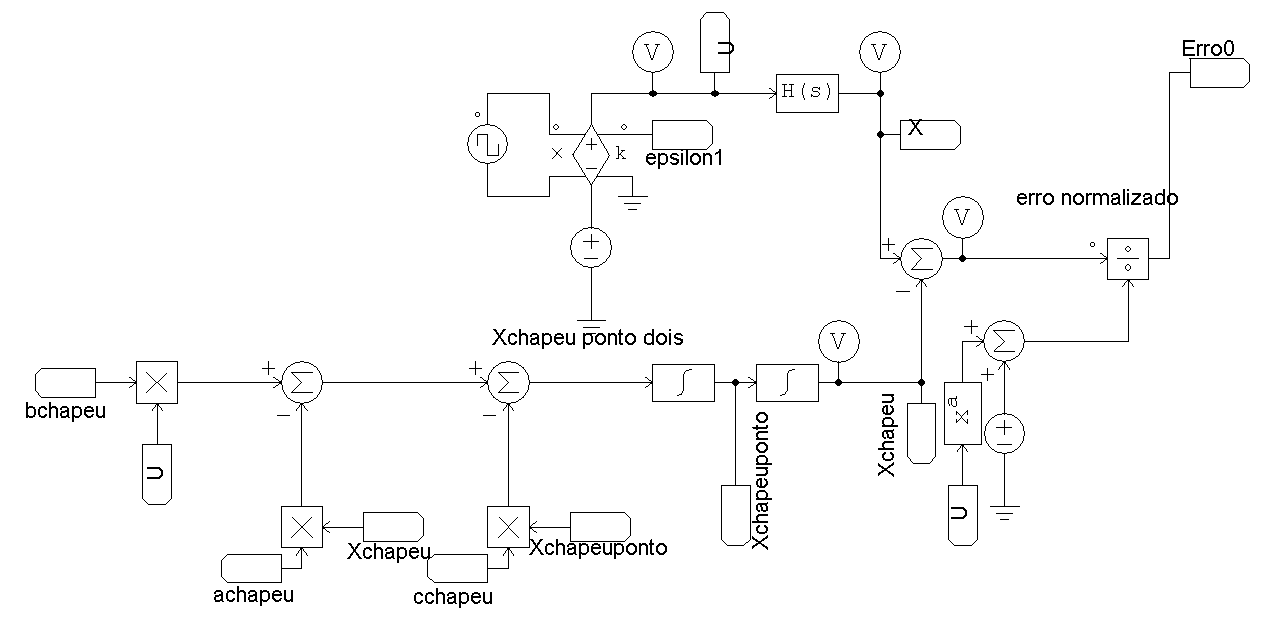
\includegraphics[width=16cm,height=14cm]{./pics/Modelos.png}
\caption[]{Diagrama de blocos da Planta alimentada por um sinal $U = 100+\epsilon_1\times S_q$ onde $S_q$ é uma onda quadrada de amplitude $100$, frequência $15Hz$ e ciclo de trabalho $0.5$ e $\epsilon_1$ é um número gerado de forma a atenuar a onda quadrada quando a atualização estiver numa taxa baixa o suficiente. Abaixo o modelo da planta construído a partir das estimativas de suas variáveis, a planta usada tem função de transferência $H_{(s)} = \frac{9999.44}{s^2+200s+9999.44} $}
\label{fig:modelos}
\end{figure}

\begin{figure}
\centering
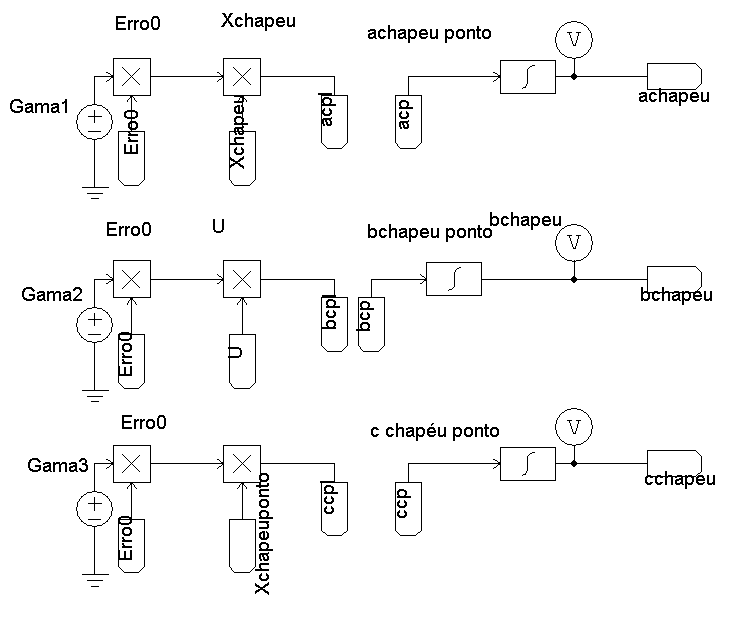
\includegraphics[width=16cm,height=14cm]{./pics/adaptacao.png}
\caption[]{Diagrama de blocos da estimação dos parâmetros da planta, os ganhos usados foram $\gamma_1 = 15000$, $\gamma_2 = 45000 $ e $\gamma_3 = 1500$, $a_{(0)} = 8000$, $b_{(0)} = 12000 $ e $c_{(0)} = 160 $}
\label{fig:estimativa}
\end{figure}

\begin{figure}
\centering
\includegraphics[width=16cm,height=14cm]{./pics/projecao.png}
\caption[]{Implementação simples do esquema de projeção para a estimação do parâmetro "a" da planta através de um "if" analógico (apenas o controle do multiplexador mostrado na figura é digital, no modelo de simulação usado no programa os sinais que o atravessam podem ser analógicos), o mesmo esquema está implementado para "b" e "c". Os limites escolhidos foram $a_{Sup} = 15000$, $a_{Inf} = 5000$, $b_{Sup} = 15000$, $b_{Inf} = 5000$, $c_{Sup} = 400$, $c_{Inf} = 75$}
\label{fig:projecao}
\end{figure}


\begin{figure}
\centering
\includegraphics[width=16cm,height=14cm]{./pics/atenuacaoPE.png}
\caption[]{Esquema de geração do número $\epsilon_1$ de forma que o sinal P.E seja atenuado quando não for mais necessário. Corresponde ao inverso da soma dos quadrados das taxas de atualização e multiplicadas por ganhos individuais. $\epsilon_1  = \frac{1}{1+\dot{\hat{a}}^2q_1+\dot{\hat{b}}^2 q_2+\dot{\hat{c}}^2q_3}$. O critério usado para a calibragem inicial dos ganhos q foi o de equalização das ordens de magnitude de cada fator, após isso reduzimos q de forma que o sinal desligue apropriadamente durante a simulação. Os ganhos finais escolhidos foram $q_1 =  0.015, q_2 = 0.006, q_3 = 0.007$}  
\label{fig:atenuação PE}
\end{figure}

\begin{figure}
\centering
\includegraphics[width=16cm,height=14cm]{./pics/ACLetraA.png}
\caption[]{Adaptação do parâmetro A}  
\label{fig:adap A}
\end{figure}

\begin{figure}
\centering
\includegraphics[width=16cm,height=14cm]{./pics/BCLetraA.png}
\caption[]{Adaptação do parâmetro B}  
\label{fig:adap B}
\end{figure}


\begin{figure}
\centering
\includegraphics[width=16cm,height=14cm]{./pics/CCLetraA.png}
\caption[]{Adaptação do parâmetro C}  
\label{fig:adap C}
\end{figure}

\begin{figure}
\centering
\includegraphics[width=16cm,height=14cm]{./pics/E0LetraA.png}
\caption[]{Erro entre a saída da planta e a saída do modelo}  
\label{fig:E0}
\end{figure}

\begin{figure}
\centering
\includegraphics[width=16cm,height=14cm]{./pics/epsilon1LetraA.png}
\caption[]{Figura de mérito para atenuação $\epsilon_1$}  
\label{fig:eps1}
\end{figure}

\begin{figure}
\centering
\includegraphics[width=16cm,height=14cm]{./pics/ULetraA.png}
\caption[]{Entrada da planta U}  
\label{fig:U}
\end{figure}


\begin{figure}
\centering
\includegraphics[width=16cm,height=14cm]{./pics/XLetraA.png}
\caption[]{Saída da planta X}  
\label{fig:X}
\end{figure}

 
\chapter*{Lista 3, Letra C}

Introduzimos a função de custo integral. O diagrama de blocos para a mesma está detalhado nas figuras 12 e 13 a seguir, os resultados se encontram nas figuras de 14 até 20. Nesta simulação usamos um passo de $10^{-3}s$. É possível melhorar os resultados da simulação alterando o passo para um valor menor e re-escolhendo os ganhos de forma a evitar erros numéricos. Desta forma obtivemos um tempo de convergência bastante lento.

\begin{figure}
\centering
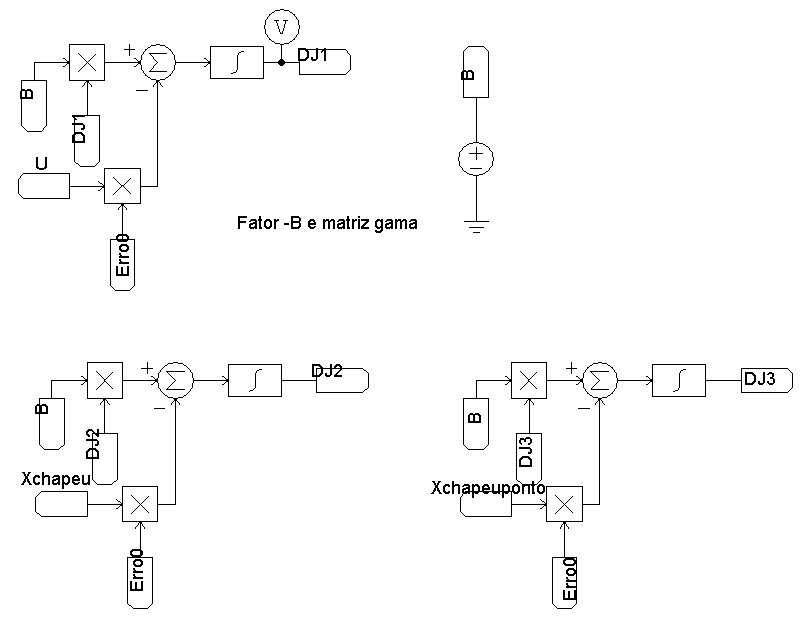
\includegraphics[width=16cm,height=14cm]{./pics/FCustoIntegrativo.png}
\caption[]{Função de custo integrativa, implementamos $\nabla J$ através do diagrama de blocos acima. Escolhemos $\beta = 2$}  
\label{fig:FCI}
\end{figure}

\begin{figure}
\centering
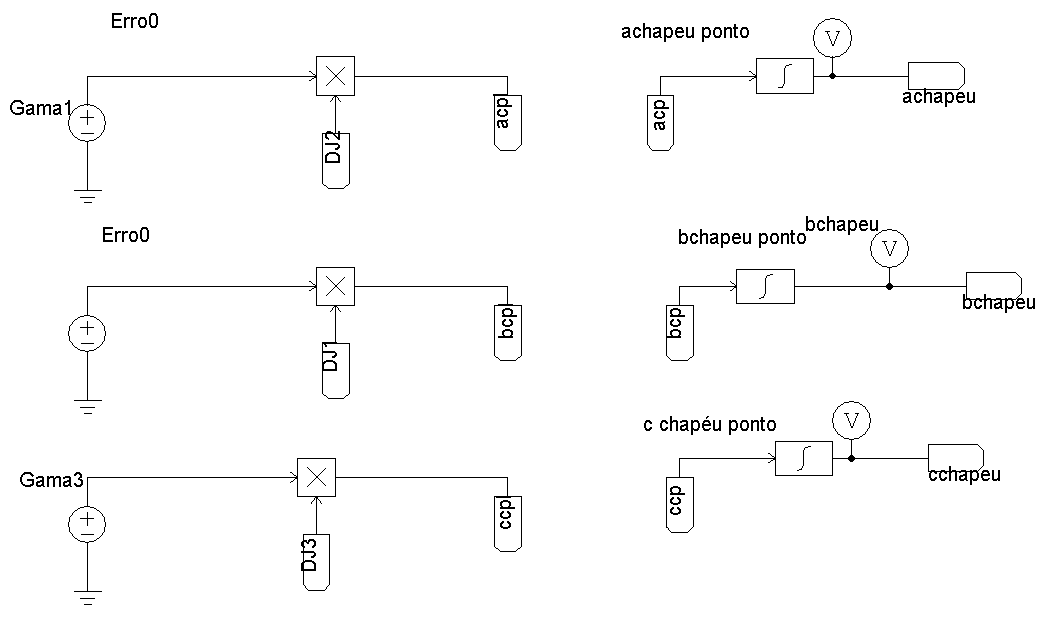
\includegraphics[width=16cm,height=14cm]{./pics/FCustoIntegrativoAdaptacao.png}
\caption[]{Nova lei adaptativa para os parâmetros "a", "b" e "c", as estimativas inicias são $a_{(0)} = 14000, b_{(0)} = 6000, c_{(0)} = 120$ e $\gamma_1 = 300$, $\gamma_2 = 250 $ e $\gamma_3 = 80$}  
\label{fig:FCIA}
\end{figure}


\begin{figure}
\centering
\includegraphics[width=16cm,height=14cm]{./pics/ACLetraC.png}
\caption[]{Adaptação do parâmetro A}  
\label{fig:adap Ac}
\end{figure}

\begin{figure}
\centering
\includegraphics[width=16cm,height=14cm]{./pics/BCLetraC.png}
\caption[]{Adaptação do parâmetro B}  
\label{fig:adap Bc}
\end{figure}


\begin{figure}
\centering
\includegraphics[width=16cm,height=14cm]{./pics/CCLetraC.png}
\caption[]{Adaptação do parâmetro C}  
\label{fig:adap Cc}
\end{figure}

\begin{figure}
\centering
\includegraphics[width=16cm,height=14cm]{./pics/E0LetraC.png}
\caption[]{Erro entre a saída da planta e a saída do modelo}  
\label{fig:E0c}
\end{figure}

\begin{figure}
\centering
\includegraphics[width=16cm,height=14cm]{./pics/epsilon1LetraC.png}
\caption[]{Figura de mérito para atenuação $\epsilon_1$}  
\label{fig:epsc1}
\end{figure}

\begin{figure}
\centering
\includegraphics[width=16cm,height=14cm]{./pics/ULetraC.png}
\caption[]{Entrada da planta U}  
\label{fig:Uc}
\end{figure}


\begin{figure}
\centering
\includegraphics[width=16cm,height=14cm]{./pics/XLetraC.png}
\caption[]{Saída da planta X}  
\label{fig:Xc}
\end{figure}



\chapter*{Lista 3, Letra E}

Fizemos a estimativa a partir do método dos mínimos quadrados porém não conseguimos obter um resultado de convergência rápido. Implementamos o método com fator de esquecimento e substituímos a reinicialização da matriz P por uma técnica de projeção simples para cada um dos ganhos da matriz, além de manter a projeção para as estimativas dos parâmetros da planta. O diagrama de blocos para estas técnicas está detalhado nas figuras 21 e 22 enquanto as figuras de 23 a 32 mostram os resultados da simulação. 


\begin{figure}
\centering
\includegraphics[width=16cm,height=14cm]{./pics/ACLetraE.png}
\caption[]{Adaptação do parâmetro A}  
\label{fig:adap AcE}
\end{figure}

\begin{figure}
\centering
\includegraphics[width=16cm,height=14cm]{./pics/BCLetraE.png}
\caption[]{Adaptação do parâmetro B}  
\label{fig:adap BcE}
\end{figure}


\begin{figure}
\centering
\includegraphics[width=16cm,height=14cm]{./pics/CCLetraE.png}
\caption[]{Adaptação do parâmetro C}  
\label{fig:adap CcE}
\end{figure}

\begin{figure}
\centering
\includegraphics[width=16cm,height=14cm]{./pics/G1LetraE.png}
\caption[]{Atualização de $\gamma_1$}  
\label{fig:adap GAcE}
\end{figure}

\begin{figure}
\centering
\includegraphics[width=16cm,height=14cm]{./pics/G2LetraE.png}
\caption[]{Atualização de $\gamma_2$}  
\label{fig:adap GBcE}
\end{figure}


\begin{figure}
\centering
\includegraphics[width=16cm,height=14cm]{./pics/G3LetraE.png}
\caption[]{Atualização de $\gamma_3$}  
\label{fig:adap GCcE}
\end{figure}

\begin{figure}
\centering
\includegraphics[width=16cm,height=14cm]{./pics/E0LetraE.png}
\caption[]{Erro entre a saída da planta e a saída do modelo}  
\label{fig:E0E}
\end{figure}

\begin{figure}
\centering
\includegraphics[width=16cm,height=14cm]{./pics/epsilon1LetraE.png}
\caption[]{Figura de mérito para atenuação $\epsilon_1$}  
\label{fig:epsE1}
\end{figure}

\begin{figure}
\centering
\includegraphics[width=16cm,height=14cm]{./pics/ULetraE.png}
\caption[]{Entrada da planta U}  
\label{fig:UE}
\end{figure}


\begin{figure}
\centering
\includegraphics[width=16cm,height=14cm]{./pics/XLetraE.png}
\caption[]{Saída da planta X}  
\label{fig:XE}
\end{figure}

